%% Offline-Verifiable Runtime Evidence Bundles for Governed AI Agent Systems
%% IEEEtran conference format. Derived from the \Argorix preprint; no new
%% experiments, metrics, citations, or deployment claims are introduced.
\documentclass[conference]{IEEEtran}
\IEEEoverridecommandlockouts

\usepackage[T1]{fontenc}
\usepackage[utf8]{inputenc}
\usepackage{cite}
\usepackage{amsmath,amssymb}
\usepackage{graphicx}
\usepackage{booktabs}
\usepackage{array}
\usepackage{xcolor}
\usepackage{listings}
\usepackage{tikz}
\usetikzlibrary{arrows.meta,positioning,fit,backgrounds,shapes.geometric,calc}
\usepackage{url}
\usepackage{xspace}
\usepackage[hidelinks]{hyperref}

% Compact monospace helper for inline identifiers/fields.
\newcommand{\code}[1]{\texttt{\small #1}}
% Breakable "<name>_digest" identifier for tight table cells: allows a line
% break after the underscore so long digest names do not overflow a column.
\newcommand{\dgst}[1]{\code{#1\_\allowbreak digest}}
% Ragged-right paragraph column for tables (avoids overfull monospace cells).
\newcolumntype{L}[1]{>{\raggedright\arraybackslash}p{#1}}

% \Argorix brand wordmark: per-character gradient across the brand palette
% (reused from the original \Argorix preprint preamble).
\definecolor{argViolet}{HTML}{7C3AED}
\definecolor{argIndigo}{HTML}{5B3DF5}
\definecolor{argElectric}{HTML}{2F6BFF}
\definecolor{argCyan}{HTML}{2BC4F4}
\definecolor{argCyanBright}{HTML}{5CD6FF}
\newcommand{\Argorix}{%
\textcolor{argViolet}{A}\textcolor{argViolet}{r}\textcolor{argIndigo}{g}\textcolor{argIndigo}{o}\textcolor{argElectric}{r}\textcolor{argElectric}{i}\textcolor{argElectric}{x}\textcolor{argCyan}{L}\textcolor{argCyan}{a}\textcolor{argCyanBright}{n}\textcolor{argCyanBright}{g}\xspace}

% Listing style for the verification algorithm.
\lstset{basicstyle=\ttfamily\scriptsize,breaklines=true,frame=single,
  columns=fullflexible,keepspaces=true,xleftmargin=0.5em}

% Shared TikZ styles for figure stubs.
\tikzset{
  ebox/.style={draw,rounded corners=2pt,align=center,inner sep=3pt,
    font=\scriptsize,minimum height=6mm},
  eimpl/.style={ebox,fill=black!4},
  eprop/.style={ebox,draw,dashed,fill=white},
  eflow/.style={-{Latex[length=2mm]},thin},
  edash/.style={-{Latex[length=2mm]},thin,dashed},
}

\begin{document}

\title{Offline-Verifiable Runtime Evidence Bundles\\for Governed AI Agent Systems}

\author{
\IEEEauthorblockN{Gustavo Venegas\IEEEauthorrefmark{1},
Edison Vazquez\IEEEauthorrefmark{1},
Danilo Naranjo\IEEEauthorrefmark{2},
Benjamin Gonzalez\IEEEauthorrefmark{1}}
\IEEEauthorblockA{\IEEEauthorrefmark{1}Chilean Chamber of Artificial Intelligence\quad
\IEEEauthorrefmark{2}Ocular\\
\texttt{\footnotesize gustavo@gobiernoia.cl,\ edison@jhedai.com,\ dan@ocularsolution.com,\ ben@nirvana-ai.com}}
}

\maketitle

\begin{abstract}
Governed AI agent runtimes emit model calls, tool decisions, provider-boundary
outcomes, and policy results, but the evidence of what happened is usually a
human-facing UI label, a provider log, or an informal status field that a consumer must
trust without independent recomputation. We present \Argorix's \emph{EvidenceBundle}, a
local runtime artifact that links a compiled bytecode program, an execution trace, a
security report, and a trace-event ledger digest through semantic SHA-256 digests
computed over canonical JSON. A verifier recomputes each digest and re-derives the
ledger digest from the trace events, then checks that the security report's
LedgerSummary digest matches the bundle, establishing cross-artifact consistency without
network access, provider credentials, a live runtime, or any external service. We give a
lightweight formal model of the verification predicate and show it is distinct from
policy approval: a bundle can verify while the security report records policy failure and
a review-required state. In an existing corpus of 33 request directories, 27 are complete
and pass offline verification (27/27); 6 are source-only and not assessable. The corpus
contains 7{,}155 counted ledger events and 1{,}188 detailed policy violations, and every
complete session records \code{policy\_passed=false}, \code{review\_required=true}. We
hold a strict interpretation boundary: successful verification proves internal artifact
consistency relative to the bundle only---not source integrity, producer authentication,
absence of side effects, policy approval, certification, or production isolation.
\end{abstract}

\begin{IEEEkeywords}
AI agents, runtime evidence, evidence bundles, offline verification, semantic digests,
canonical JSON, agent governance, auditability, policy evidence, reproducibility.
\end{IEEEkeywords}

\section{Introduction}\label{sec:intro}
A governed AI agent does not execute in a vacuum. A single request can issue model
calls, invoke tools, cross a provider boundary, trigger policy evaluation, and produce a
verdict. \emph{Governance} means a downstream party---an auditor, an operator, a
compliance reviewer, or a second agent---must later determine what the runtime actually
did. The difficulty is that the evidence on offer is almost always \emph{mediated}: a
dashboard renders a green checkmark, a provider returns an opaque log line, a human
writes ``reviewed---OK'' into a status field. Each is a summary produced by a party the
consumer must already trust, and none can be independently recomputed from the artifacts
themselves.

This is unsatisfactory for governed deployments for three reasons. First, a favorable
\emph{summary} can mask an unfavorable \emph{underlying} result: a top-level ``checks
passed'' banner says nothing about whether a detailed policy object recorded a violation.
Second, evidence tied to a \emph{live} service is unavailable precisely when it is most
needed---after the fact, offline, when the provider is gone or uncooperative. Third, a
mediated label conflates distinct predicates---\emph{did the artifacts survive
unchanged?} and \emph{was the behavior approved?}---that governance requires be kept
apart.

We argue that runtime evidence for governed agents must instead be (i) \emph{inspectable
after execution}, as concrete artifacts on disk; (ii) \emph{verifiable without a live
provider}, using only local recomputation; and (iii) \emph{claim-bounded}, so that what
verification establishes is never silently promoted into what it does not. \Argorix
\cite{venegas2026argorixlang,argorixlang2026} realizes this with the
\emph{EvidenceBundle}: a local artifact that records semantic SHA-256 digests of a
compiled bytecode program, an execution trace, and a security report, plus a digest of
the trace-event ledger, together with a relative-path artifact map. A verifier loads the
referenced artifacts, recomputes every digest over canonical JSON, re-derives the ledger
digest from the trace events, and checks that the report's embedded LedgerSummary digest
matches the bundle---with no network, no credential, and no external service.

The central stance of this paper, and its central claim boundary, is that
\emph{artifact integrity is not policy approval}. A verified bundle proves only that the
bytecode, trace, and report are mutually consistent relative to the bundle. It does not
prove that the source compiled to that bytecode, who produced the bundle, that no side
effects occurred outside instrumentation, or that any policy approved the behavior. We
make this separation formal (Section~\ref{sec:formal}) and show that the existing corpus
contains cases that are \emph{verifiable and policy-failing simultaneously}
(Section~\ref{sec:eval}).

\noindent\textbf{Contributions.}
\begin{enumerate}
\item A runtime evidence model for governed AI agent systems, expressed as concrete
on-disk artifacts rather than mediated summaries.
\item A semantic-digest \emph{bundle} linking bytecode, trace, security report, and a
trace-event ledger digest over canonical JSON.
\item A formal \emph{offline verification predicate} over those artifacts, with an
accompanying verification algorithm requiring no live service.
\item A formal \emph{interpretation boundary} separating EvidenceBundle verification from
policy approval, stated as $\mathrm{Verify}\nRightarrow\mathrm{PolicyApproved}$.
\item An \emph{observational evaluation} using the existing \Argorix runtime corpus,
reporting what the evidence does and does not establish.
\end{enumerate}

A scope note distinguishing this paper from the companion Agent Passport paper is given
in Section~\ref{sec:diff}.

\begin{figure*}[t]
\centering
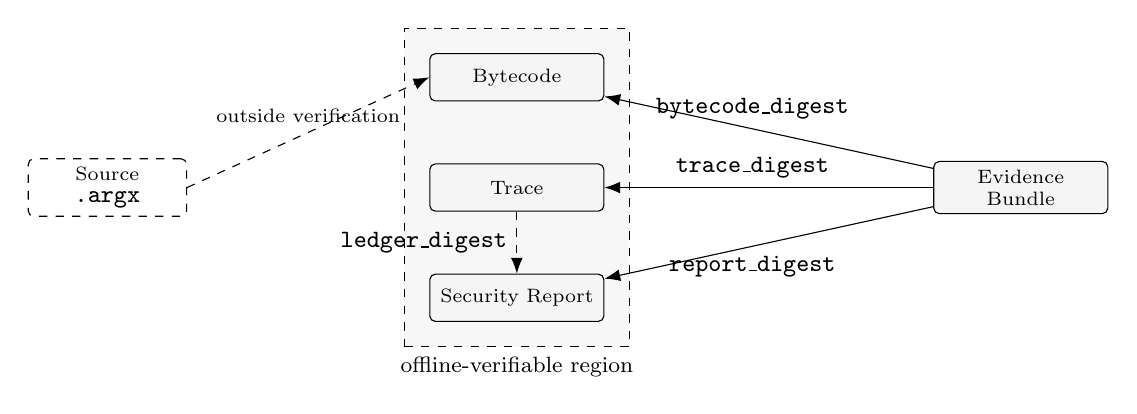
\begin{tikzpicture}[every node/.style={font=\footnotesize}]
% left: source, outside the verification boundary
\node[eprop,text width=18mm] (src) at (0,1.0) {Source\\\code{.argx}};
% middle: the three pinned artifacts
\node[eimpl,text width=20mm] (bc) at (5.2,2.4) {Bytecode};
\node[eimpl,text width=20mm] (tr) at (5.2,1.0) {Trace};
\node[eimpl,text width=20mm] (sr) at (5.2,-0.4) {Security Report};
% right: the evidence bundle that pins them
\node[eimpl,text width=20mm] (eb) at (11.6,1.0) {Evidence Bundle};
% source -> bytecode: outside bundle verification (dashed)
\draw[edash] (src.east) -- node[midway,above,font=\scriptsize]{outside verification} (bc.west);
% bundle pins each artifact via a semantic digest
\draw[eflow] (eb) -- node[pos=0.55,above,font=\scriptsize]{\dgst{bytecode}} (bc);
\draw[eflow] (eb) -- node[pos=0.55,above,font=\scriptsize]{\dgst{trace}} (tr);
\draw[eflow] (eb) -- node[pos=0.55,below,font=\scriptsize]{\dgst{report}} (sr);
% ledger digest: derived from trace.events, matched against the report
\draw[edash] (tr) -- node[midway,left,font=\scriptsize]{\dgst{ledger}} (sr);
\begin{scope}[on background layer]
\node[draw,dashed,fill=black!3,fit=(bc)(tr)(sr),inner sep=9pt,
  label=below:{\footnotesize offline-verifiable region}] {};
\end{scope}
\end{tikzpicture}
\caption{Evidence artifact graph. The source lies outside the verification boundary
(dashed edge). Bytecode, trace, and security report form the offline-verifiable region;
the Evidence Bundle pins each via a semantic digest, and the ledger digest---derived from
\code{trace.events}---is matched against the report's LedgerSummary.}
\label{fig:graph}
\end{figure*}

\section{Background and Motivation}\label{sec:background}

\subsection{What an agent runtime produces}
A governed agent runtime emits a heterogeneous record: model invocations, tool-call
decisions, provider-boundary crossings (or refusals), policy evaluations, and a final
verdict. \Argorix serializes this record into four artifact \emph{kinds} downstream of an
upstream source program: a compiled bytecode program, an ordered execution trace, a
structured security report, and an evidence bundle that ties them together. The
distinction between kinds matters because they play different evidential roles.

\subsection{Logs, reports, provenance, attestation, bundles}
These terms should not be used interchangeably. A \emph{log} is an append-only stream,
typically unverifiable after the fact and trusted by provenance of the emitter. A
\emph{report} is an interpretation: a structured judgment over a run. A \emph{provenance
record} asserts how an artifact was produced and, in signed forms (e.g., in-toto
\cite{torresarias2019intoto}), binds that assertion to a key. An \emph{attestation} is a
signed statement by an identified party. An \emph{evidence bundle}, as used here, is none
of these: it is an \emph{unsigned, local, recomputable cross-artifact consistency
record}. It states that specific artifacts hash to given values and agree with one
another, and nothing about who produced them.

\subsection{Why digest verification helps but is not trust}
A semantic digest detects \emph{change relative to a recorded value}. If a verifier
recomputes $H(bc)$ and it matches \code{B.bytecode\_digest}, the bytecode is the one the
bundle recorded. This is genuinely useful: it makes silent tampering of a self-contained
bundle detectable, reproducibly and offline. But it establishes nothing about
\emph{origin}---an adversary who controls artifacts and bundle together can produce a
self-consistent bundle with attacker-chosen content. Digest verification is a
consistency primitive, not a trust primitive.

\subsection{Why policy evidence must preserve failure}
An evidence system is only useful if it faithfully preserves negative results. The
temptation in agent UIs is to collapse a run into a single optimistic status. \Argorix's
security report instead retains detailed policy objects---per-block results, violations,
and a \code{review\_required} flag---so that a favorable coarse label cannot overwrite a
detailed failure. Preserving the negative is the point: an auditor needs to see the
violation, not a smoothed-over banner.

\subsection{Relation to adjacent systems}
in-toto \cite{torresarias2019intoto} provides \emph{signed} supply-chain provenance;
EvidenceBundles are local and unsigned. OPA \cite{opa_docs} is an external policy
\emph{decision} engine; \Argorix records policy outcomes inside runtime artifacts rather
than externalizing the decision. WASI \cite{wasi_intro} provides capability isolation at
the host; bundle verification proves nothing about host sandboxing. MCP and A2A
\cite{mcp_spec_2025,a2a_spec} standardize agent interaction surfaces; bundles record
local runtime boundaries, not live interoperability. The NIST AI RMF
\cite{tabassi2023airmf} and the OWASP Top 10 for LLM Applications
\cite{owasp_llm_top10} frame risk and inform our threat discussion, but neither is a
certification we claim to satisfy.

\section{Evidence Artifact Model}\label{sec:model}
We define each artifact and fix its verification scope; Table~\ref{tab:artifacts}
summarizes.

\emph{(1) Source} (\code{session.argx}) is the upstream compiler input. It is
\emph{outside} bundle verification: the bundle carries no source path and no source
digest, so verification begins at compiled bytecode and never asserts that the source
produced it.

\emph{(2) Bytecode} (\code{session.argbc.json}) is the compiled program loaded by the VM,
verified by \code{bytecode\_digest}; cross-checks on \code{language}, \code{module}, and
\code{bytecode\_version} guard against gross substitution.

\emph{(3) Trace} (\code{session.trace.json}) is an ordered ledger of runtime and policy
events---agent and policy declarations, message scheduling/delivery, handler execution,
policy evaluations, and VM lifecycle markers---verified by \code{trace\_digest} and the
source of the ledger digest.

\emph{(4) SecurityReport} (\code{session.security.json}) is a structured interpretation
of runtime state: execution status, policy outcomes (\code{passed}, \code{violations},
\code{review\_required}), provider boundary, call counts, and a verdict. It is verified
by \code{report\_digest} and contains a \emph{LedgerSummary} whose \code{ledger\_digest}
must equal the bundle's.

\emph{(5) EvidenceBundle} (\code{session.evidence.json}) holds the artifact map plus four
semantic digests (\code{bytecode\_digest}, \code{trace\_digest}, \code{report\_digest},
\code{ledger\_digest}). The artifact map (\code{bytecode\_path}, \code{trace\_path},
\code{security\_report\_path}) holds \emph{relative} paths confined to the bundle's
portable subtree; there is no source path and no standalone ledger path.

\emph{(6) Ledger digest} is computed as $H(\mathrm{events}(tr))$---the canonical digest
of the trace's event list, not a separate file. It is checked against the bundle's
\code{ledger\_digest} \emph{and} the report's embedded LedgerSummary digest, binding the
trace's events to the report's claims about them.

\noindent\textbf{Scope, stated plainly.} The bundle's verifiable region \emph{starts} at
bytecode, trace, and report. It does not verify that \code{session.argx} produced the
bytecode; it does not authenticate who produced the bundle; and it does not prove
security, compliance, or absence of effects.

\begin{table}[t]
\centering
\caption{Runtime evidence artifacts.}
\label{tab:artifacts}
\renewcommand{\arraystretch}{1.25}
\scriptsize
\setlength{\tabcolsep}{3pt}
\begin{tabular}{@{}L{0.13\columnwidth}L{0.18\columnwidth}L{0.15\columnwidth}L{0.24\columnwidth}L{0.16\columnwidth}@{}}
\toprule
\textbf{Artifact} & \textbf{Path} & \textbf{Role} & \textbf{Verified by} & \textbf{Out-of-scope} \\
\midrule
Source & \code{.argx} & Compiler input & --- (not in bundle) & Source$\to$\allowbreak bytecode link \\
Bytecode & \code{.argbc\allowbreak.json} & Compiled program & \dgst{bytecode} & Source provenance \\
Trace & \code{.trace\allowbreak.json} & Event ledger & \dgst{trace}, \dgst{ledger} & Un\-in\-stru\-mented events \\
Sec.\ Report & {\scriptsize\texttt{.security\allowbreak.json}} & Runtime/\allowbreak policy interp.\ & \dgst{report}; LS match & Truth of metadata \\
Evidence Bundle & {\scriptsize\texttt{.evidence\allowbreak.json}} & Map + digests & cross-checked & Producer identity \\
Ledger digest & (from \code{trace\allowbreak.events}) & Binds events to report & $H(\mathrm{events}(tr))$ & Standalone ledger \\
\bottomrule
\end{tabular}
\end{table}

\section{Formal Model}\label{sec:formal}
We give a lightweight formalization. It is an \emph{interpretation boundary}, not a
cryptographic security proof.

\noindent\textbf{Definitions.} Let $B$ be an EvidenceBundle; $bc$, $tr$, $sr$ the
bytecode, trace, and security-report artifacts; $\mathrm{events}(tr)$ the ordered trace
event list; $\mathrm{LS}(sr)$ the LedgerSummary digest stored in the report; $C(x)$ the
canonical JSON serialization of $x$; and $H(x)=\mathrm{SHA\text{-}256}(C(x))$.

\noindent\textbf{Semantic-digest equations.}
\begin{align}
B.\textsf{bytecode\_digest} &= H(bc) \\
B.\textsf{trace\_digest}    &= H(tr) \\
B.\textsf{report\_digest}   &= H(sr) \\
B.\textsf{ledger\_digest}   &= H(\mathrm{events}(tr)) \\
\mathrm{LS}(sr)             &= B.\textsf{ledger\_digest}
\end{align}

\noindent\textbf{Verification predicate.}
\begin{align*}
\mathrm{Verify}(B,bc,tr,sr) :=\ &
B.\textsf{bytecode\_digest} = H(bc) \\
\wedge\ & B.\textsf{trace\_digest} = H(tr) \\
\wedge\ & B.\textsf{report\_digest} = H(sr) \\
\wedge\ & B.\textsf{ledger\_digest} = H(\mathrm{events}(tr)) \\
\wedge\ & \mathrm{LS}(sr) = B.\textsf{ledger\_digest}
\end{align*}

\noindent\textbf{Policy approval (a separate predicate).}
\begin{align*}
\mathrm{PolicyApproved}(sr) :=\ &
sr.\textsf{policy\_passed} = \mathrm{true} \\
\wedge\ & sr.\textsf{review\_required} = \mathrm{false} \\
\wedge\ & |sr.\textsf{violations}| = 0
\end{align*}

\noindent\textbf{Interpretation boundary (central result).} Verification does not imply
approval:
\[
\mathrm{Verify}(B,bc,tr,sr)\ \nRightarrow\ \mathrm{PolicyApproved}(sr).
\]
The predicates read disjoint fields: $\mathrm{Verify}$ reads digests and the
LedgerSummary; $\mathrm{PolicyApproved}$ reads \code{policy\_passed},
\code{review\_required}, and \code{violations}. Nothing in $\mathrm{Verify}$ constrains
the latter, so a faithfully recorded policy failure passes through verification
unchanged. The observed corpus witnesses the satisfiable conjunction
\[
\exists\, sr:\ \mathrm{Verify}(B,bc,tr,sr)\ \wedge\ \neg\mathrm{PolicyApproved}(sr),
\]
because complete bundles verify (27/27) while their reports record
\code{policy\_passed=false} and \code{review\_required=true}. We do \emph{not} present
$\mathrm{Verify}$ as proof of authenticity, source integrity, or external truth; it is a
statement of internal cross-artifact consistency relative to $B$.
Table~\ref{tab:predicates} restates these predicates.

\begin{table}[t]
\centering
\caption{Formal predicates.}
\label{tab:predicates}
\renewcommand{\arraystretch}{1.3}
\scriptsize
\setlength{\tabcolsep}{3pt}
\begin{tabular}{@{}L{0.30\columnwidth}L{0.30\columnwidth}L{0.28\columnwidth}@{}}
\toprule
\textbf{Predicate} & \textbf{Definition} & \textbf{Interpretation} \\
\midrule
$H(x)$ & $\mathrm{SHA\text{-}256}(C(x))$ & Semantic digest over canonical JSON \\
$\mathrm{Verify}$ & five digest/LS equalities hold & Internal consistency relative to $B$ \\
$\mathrm{PolicyApproved}$ & passed $\wedge$ $\neg$review $\wedge$ no violations & Approval as recorded by the report \\
$\mathrm{Verify}$ $\nRightarrow$ $\mathrm{PolicyApproved}$ & verification $\neq$ approval & Integrity boundary (central) \\
$\exists:$ $\mathrm{Verify}$ $\wedge$ $\neg\mathrm{PolicyApproved}$ & witnessed by corpus & 27/27 verify while failing \\
\bottomrule
\end{tabular}
\end{table}

\section{Offline Verification Procedure}\label{sec:verify}
The verifier is a pure function of local files. It loads the bundle; resolves
\code{bytecode\_path}, \code{trace\_path}, and \code{security\_report\_path} relative to
the bundle directory (rejecting absolute paths and paths escaping the portable subtree);
loads the three artifacts; canonicalizes each to JSON; recomputes \code{bytecode\_digest},
\code{trace\_digest}, and \code{report\_digest}; recomputes \code{ledger\_digest} from
\code{trace.events}; compares the report's LedgerSummary digest against the bundle's; and
returns \emph{verified} only if all checks pass. It requires \emph{no network access, no
provider credential, no live runtime, and no external service}. Auxiliary checks
(version-field agreement across artifacts, digest well-formedness, path confinement)
accompany the core comparisons.

\begin{figure}[t]
\lstset{caption={},label={}}
\begin{lstlisting}
Algorithm 1: Offline EvidenceBundle Verification
Input : bundle file B (referencing bc, tr, sr)
Output: verified in {true, false}

 1. Load B.
 2. Resolve B.artifact_map paths
    (relative, inside portable tree).
 3. Load bc, tr, sr.
 4. d_bc     <- H(bc)
 5. d_tr     <- H(tr)
 6. d_sr     <- H(sr)
 7. d_ledger <- H(events(tr))
 8. check d_bc     = B.bytecode_digest
 9. check d_tr     = B.trace_digest
10. check d_sr     = B.report_digest
11. check d_ledger = B.ledger_digest
12. check LS(sr)   = B.ledger_digest
13. return verified iff checks (8)-(12) all hold
\end{lstlisting}
\caption{Offline verification recomputes every digest from local artifacts and compares
against the bundle; no live service participates.}
\label{fig:algo}
\end{figure}

\begin{figure}[t]
\centering
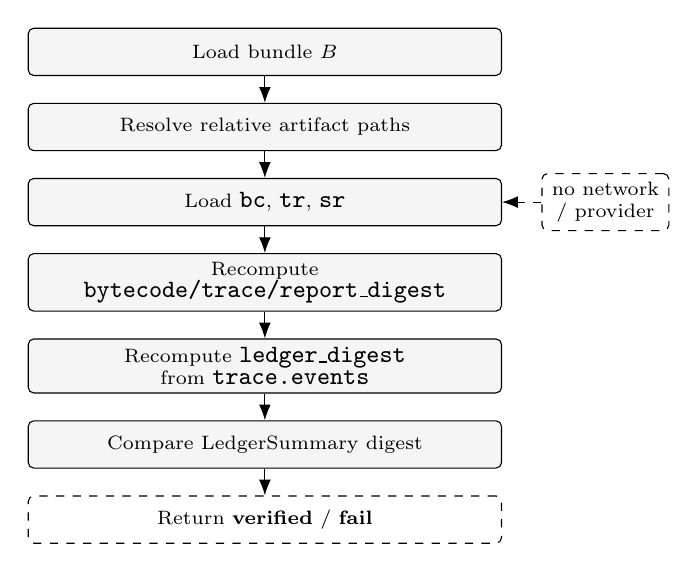
\begin{tikzpicture}[node distance=3.4mm,every node/.style={font=\scriptsize}]
\node[eimpl,text width=58mm] (s1) {Load bundle $B$};
\node[eimpl,below=of s1,text width=58mm] (s2) {Resolve relative artifact paths};
\node[eimpl,below=of s2,text width=58mm] (s3) {Load \code{bc}, \code{tr}, \code{sr}};
\node[eimpl,below=of s3,text width=58mm] (s4) {Recompute \code{bytecode/trace/report\_digest}};
\node[eimpl,below=of s4,text width=58mm] (s5) {Recompute \code{ledger\_digest} from \code{trace.events}};
\node[eimpl,below=of s5,text width=58mm] (s6) {Compare LedgerSummary digest};
\node[eprop,below=of s6,text width=58mm] (s7) {Return \textbf{verified} / \textbf{fail}};
\draw[eflow] (s1)--(s2); \draw[eflow] (s2)--(s3); \draw[eflow] (s3)--(s4);
\draw[eflow] (s4)--(s5); \draw[eflow] (s5)--(s6); \draw[eflow] (s6)--(s7);
\node[eprop,right=5mm of s3,text width=14mm] (net) {no network / provider};
\draw[edash] (net) -- (s3);
\end{tikzpicture}
\caption{Offline verification sequence. Every step reads local files only; no provider
or network participates.}
\label{fig:seq}
\end{figure}

\section{Integrity Is Not Approval}\label{sec:integrity}
This section is the conceptual core. Six statements bound what a verified bundle means.
\emph{(1) Consistency, not external truth:} a valid bundle proves the artifacts agree
relative to the bundle, not that any claim they make is externally true. \emph{(2) Change
detection, not origin:} a matching digest detects change relative to a recorded artifact,
not who produced it; an unsigned bundle has no producer binding. \emph{(3) Instrumented
events, not all events:} a verified trace records instrumented events faithfully but
cannot prove that no effect occurred outside the instrumentation boundary.
\emph{(4) Faithful negatives:} a verified report can preserve a negative policy result
without contradiction; verifying the report is orthogonal to the report's verdict.
\emph{(5) Detail dominates summary:} a favorable top-level status must not override a
detailed policy failure---component status and \code{review\_required} dominate
interpretation. \emph{(6) The central statement:} \emph{a bundle can be offline-verifiable
and still contain policy failure, a review-required status, unknown-rule violations, or
otherwise non-certified behavior.} Table~\ref{tab:vsapproval} tabulates the distinction
across specific claims.

\begin{table}[t]
\centering
\caption{Integrity vs.\ approval distinction.}
\label{tab:vsapproval}
\renewcommand{\arraystretch}{1.25}
\scriptsize
\setlength{\tabcolsep}{3pt}
\begin{tabular}{@{}L{0.46\columnwidth}L{0.14\columnwidth}L{0.28\columnwidth}@{}}
\toprule
\textbf{Claim} & \textbf{Supported?} & \textbf{Reason} \\
\midrule
Artifacts unchanged relative to bundle & Yes & Digests recompute and match \\
Trace events match report LedgerSummary & Yes & $H(\mathrm{events}(tr))=\mathrm{LS}(sr)$ \\
Source produced this bytecode & No & No source path/digest in bundle \\
A known party produced the bundle & No & Unsigned; no producer binding \\
No side effects outside instrumentation & No & Trace sees instrumented events only \\
Policy approved the behavior & No & Separate predicate; corpus fails \\
Legal/compliance certification & No & No certification mechanism \\
Host/production isolation & No & No sandbox measurement \\
\bottomrule
\end{tabular}
\end{table}

\section{Observational Evaluation}\label{sec:eval}
We reuse the existing \Argorix runtime corpus \cite{venegas2026argorixlang} and add no
new experiment.

\subsection{Corpus}
Of \textbf{33} request directories, \textbf{27} are \emph{complete}---each containing
\code{session.argx}, \code{session.argbc.json}, \code{session.trace.json},
\code{session.security.json}, and \code{session.evidence.json}---and \textbf{6} are
\emph{source-only} and not assessable for trace/security/evidence fields. The corpus
contains \textbf{7{,}155} counted ledger events and \textbf{1{,}188} detailed policy
violations across the complete sessions.

\subsection{Offline verification}
All \textbf{27/27} complete bundles pass offline verification: the three semantic digests
reproduce, the ledger digest recomputes from \code{trace.events}, and the LedgerSummary
digest matches the bundle. No bundle digests or verifies \code{session.argx}.

\subsection{Policy results}
Every one of the 27 detailed policy reports sets \code{policy\_passed=false} and
\code{review\_required=true}, with \textbf{44} unknown-rule violations per complete
session. Verification success therefore coexists with policy non-approval---the witnessed
conjunction of Section~\ref{sec:formal}. Table~\ref{tab:corpus} summarizes.

\begin{table}[t]
\centering
\caption{Observational corpus results.}
\label{tab:corpus}
\renewcommand{\arraystretch}{1.2}
\footnotesize
\begin{tabular}{@{}p{0.44\columnwidth}p{0.16\columnwidth}p{0.28\columnwidth}@{}}
\toprule
\textbf{Measure} & \textbf{Observed} & \textbf{Interpretation} \\
\midrule
Request directories & 33 & Full corpus \\
Complete directories & 27 & Assessable for fields \\
Source-only directories & 6 & Explicitly incomplete \\
Bundles passing offline verif.\ & 27/27 & Internal consistency only \\
Counted ledger events & 7{,}155 & Structured event emission \\
Detailed policy violations & 1{,}188 & Negatives preserved \\
Unknown-rule violations / session & 44 & Per-session failure detail \\
Reports \code{policy\_passed=false} & 27/27 & $\mathrm{Verify}\nRightarrow\mathrm{Approved}$ \\
Reports \code{review\_required=true} & 27/27 & Review state preserved \\
\bottomrule
\end{tabular}
\end{table}

\subsection{Interpretation}
The evidence pipeline is reproducible across complete sessions, and offline verification
works for every complete bundle. Missing artifacts surface as explicit incomplete
observations, not silent passes---a source-only directory is \emph{unavailable}, never
\emph{verified}. Verification success does not imply policy success. The repeated
structure supports pipeline reproducibility but limits any claim of behavioral diversity.

\begin{figure}[t]
\centering
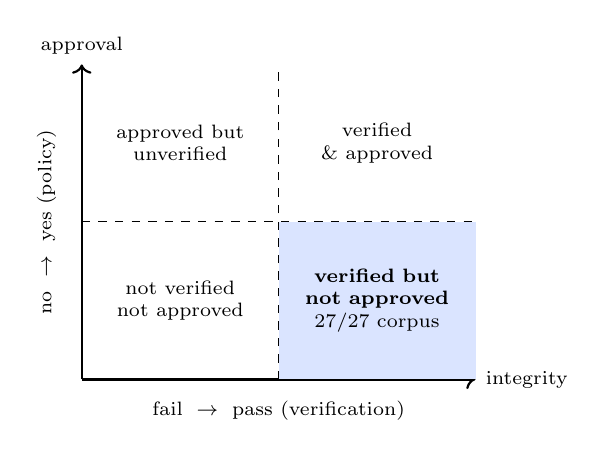
\begin{tikzpicture}[font=\scriptsize]
\draw[->,thick] (0,0) -- (5,0) node[right]{integrity};
\draw[->,thick] (0,0) -- (0,4) node[above]{approval};
\node[below] at (2.5,-0.15) {fail \;$\rightarrow$\; pass (verification)};
\node[rotate=90,above] at (-0.2,2) {no \;$\rightarrow$\; yes (policy)};
% quadrant shading: verified but not approved (lower-right)
\fill[argElectric!18] (2.5,0) rectangle (5,2);
\node[align=center,text width=22mm] at (3.75,1) {\textbf{verified but\\not approved}\\\scriptsize 27/27 corpus};
\node[align=center,text width=18mm] at (3.75,3) {\scriptsize verified\\\& approved};
\node[align=center,text width=18mm] at (1.25,1) {\scriptsize not verified\\not approved};
\node[align=center,text width=18mm] at (1.25,3) {\scriptsize approved but\\unverified};
\draw[dashed] (2.5,0)--(2.5,4);
\draw[dashed] (0,2)--(5,2);
\end{tikzpicture}
\caption{Two-axis interpretation. The corpus populates the verified-but-not-approved
quadrant: every complete session is offline-verifiable yet records policy failure---the
visual statement of $\mathrm{Verify}\nRightarrow\mathrm{PolicyApproved}$.}
\label{fig:quadrant}
\end{figure}

\section{Threat Model and Security Analysis}\label{sec:threat}
We analyze threats as attack paths across trust boundaries, not as proof that a control
defeats every adversary.

\noindent\textbf{Threats.} \emph{Artifact tampering} (altering bytecode, trace, or report
after the fact); \emph{bundle replacement} (swapping the bundle); \emph{report/status
confusion} (reading a coarse status and missing a detailed failure); \emph{missing source
integrity} (no link from bytecode back to \code{session.argx}); \emph{producer
impersonation}; \emph{unsigned bundle replay}; \emph{runtime side effects outside
instrumentation}; \emph{consumer overinterpretation} (treating consistency as
certification); and \emph{malicious but self-consistent bundle generation} (an adversary
controlling all artifacts emits a coherent bundle with chosen content).

\noindent\textbf{Bounded mitigations.} Semantic-digest linkage detects post-hoc change to
a recorded artifact; the ledger digest derived from trace events ties events to the
report's LedgerSummary; cross-artifact consistency checks (version-field agreement, path
confinement) catch mismatched substitution; explicit incomplete-session handling prevents
missing artifacts from masquerading as passes; component-level policy status and
\code{review\_required} are preserved; and the procedure is offline-reproducible.

\noindent\textbf{Remaining gaps.} There are \emph{no} signatures, \emph{no} trusted
timestamp, \emph{no} transparency log, \emph{no} source digest, \emph{no} hardware root,
\emph{no} independent witness, \emph{no} OS-level sandbox proof, \emph{no} producer
authentication, and \emph{no} revocation or witness model. Tampering and replacement are
defeated only when the adversary cannot also rewrite the bundle; against an adversary who
controls artifact and bundle together, self-consistency is necessary but not sufficient
for trust. The strongest supported statement is conditional: within the recorded artifact
set, complete bundles are offline-consistent and policy negatives are preserved. Trust
outside that set is unmeasured.

\section{Related Work}\label{sec:related}
We compare carefully and claim no equivalence. in-toto \cite{torresarias2019intoto}
provides signed supply-chain provenance binding steps to keys; \Argorix EvidenceBundles
are local, unsigned runtime-evidence records with no producer binding. OPA
\cite{opa_docs} is an external policy decision engine evaluating Rego; \Argorix records
policy and evidence outcomes in runtime artifacts rather than externalizing the decision.
WASI \cite{wasi_intro} provides capability-based host isolation; evidence verification
proves nothing about host sandboxing. MCP and A2A \cite{mcp_spec_2025,a2a_spec}
standardize agent interaction and interoperability; EvidenceBundles record local runtime
boundaries, not live interaction. The NIST AI RMF \cite{tabassi2023airmf} and the OWASP
Top 10 for LLM Applications \cite{owasp_llm_top10} provide risk framing that motivates the
threat model; we map to neither as a certification. The bundle sits in the lineage of
provenance and reproducibility systems but trades signatures and trust anchors for
offline recomputability and a strict claim boundary. The \Argorix implementation is in
Rust \cite{rust_project}.

\begin{table}[t]
\centering
\caption{EvidenceBundle digest fields.}
\label{tab:digests}
\renewcommand{\arraystretch}{1.25}
\scriptsize
\setlength{\tabcolsep}{3pt}
\begin{tabular}{@{}L{0.22\columnwidth}L{0.20\columnwidth}L{0.22\columnwidth}L{0.22\columnwidth}@{}}
\toprule
\textbf{Digest field} & \textbf{Computed from} & \textbf{Purpose} & \textbf{Does not prove} \\
\midrule
\dgst{bytecode} & $H(bc)$ & Pin compiled program & Source produced bytecode \\
\dgst{trace} & $H(tr)$ & Pin trace artifact & Instrumentation complete \\
\dgst{report} & $H(sr)$ & Pin security report & Truth of verdict \\
\dgst{ledger} & $H(\mathrm{events}(tr))$ & Bind events to LedgerSummary & Events outside trace \\
\bottomrule
\end{tabular}
\end{table}

\section{Limitations}\label{sec:limits}
We state limitations strictly. There is \emph{no} source integrity (no source digest, no
bytecode-to-source link); \emph{no} producer authentication; \emph{no} signatures;
\emph{no} trusted timestamp; \emph{no} transparency log; \emph{no} blockchain
immutability; \emph{no} post-quantum security; \emph{no} policy-approval guarantee;
\emph{no} legal or compliance certification; \emph{no} host-level containment proof;
\emph{no} controlled adversarial test; \emph{no} prompt-level qualitative analysis (prompt
content is unavailable in the corpus); \emph{no} proof of semantic correctness of every
trace event; and \emph{no} proof of absence of side effects outside the instrumented
runtime. The complete sessions are structurally uniform, supporting reproducibility but
limiting generalization across prompts, policies, and jurisdictions.

\section{Future Work}\label{sec:future}
Natural extensions, none claimed as present: source-digest inclusion so verification
extends to \code{session.argx}; signed EvidenceBundles for producer authentication and
non-repudiation; a transparency log for independent witnessing; trusted timestamps;
producer identity binding; an independent witness service; policy-decision
canonicalization into a single tri-state decision from typed component results;
differential verification across runtime versions; host-level sandbox measurement; a
controlled adversarial corpus; a public reproducibility package; and an independent
external verifier implementation.

\section{Conclusion}\label{sec:conclusion}
Offline-verifiable EvidenceBundles provide a reproducible integrity layer for governed AI
agent runtimes. They link bytecode, trace, security report, and a trace-event ledger
digest through semantic digests over canonical JSON, and a verifier re-establishes that
linkage with no live service. Their value must be read narrowly: artifact consistency,
trace/report linkage, faithful policy-result preservation, and offline auditability---not
security certification, policy approval, or external truth. The corpus shows the pipeline
is reproducible (27/27 complete bundles verify) and, decisively, that verification and
approval are distinct predicates: every complete session verifies while recording policy
failure and a review-required state.

\section{Scope}\label{sec:diff}
This paper differs from the companion Agent Passport paper by focusing on the runtime
evidence and offline verification mechanism rather than sovereign metadata. The Agent
Passport paper concerns \emph{what} metadata---country, jurisdiction, residency, policy
bindings, local agent name---is compiled and preserved; this paper concerns \emph{how}
bytecode, trace, report, and ledger evidence are linked through semantic digests and
verified offline, and where the resulting integrity claim stops. All empirical values are
reused from the original \Argorix corpus \cite{venegas2026argorixlang}, and no new
experiment, deployment, or security guarantee is introduced.

\bibliographystyle{IEEEtran}
\bibliography{references}

\end{document}
